%!TEX root = ../template.tex
%%%%%%%%%%%%%%%%%%%%%%%%%%%%%%%%%%%%%%%%%%%%%%%%%%%%%%%%%%%%%%%%%%%
%% chapter1.tex
%% NOVA thesis document file
%%
%% Chapter with introduction
%%%%%%%%%%%%%%%%%%%%%%%%%%%%%%%%%%%%%%%%%%%%%%%%%%%%%%%%%%%%%%%%%%%

% NOTE: Cite \cite{novathesis-manual} somewhere, in your thesis/dissertation with “\verb!\cite{novathesis-manual}!”, any place you think it makes sense.  If you cite it this way, the correct entry will be added automatically to your bibliography (there no need to add it to your BibTeX file);

\typeout{NT FILE chapter1.tex}

% epigraph configuration
% \epigraphfontsize{\small\itshape}
% \setlength\epigraphwidth{12.5cm}
% \setlength\epigraphrule{0pt}

% \epigraph{
%   This work is licensed under the \href{LaTeX project public license}{\LaTeX\ Project Public License v1.3c}.
%   To view a copy of this license, visit \url{LaTeX project public license}.
% }

\chapter{Introduction}\label{cha:introduction}

\begin{figure}[H]
  \centering
	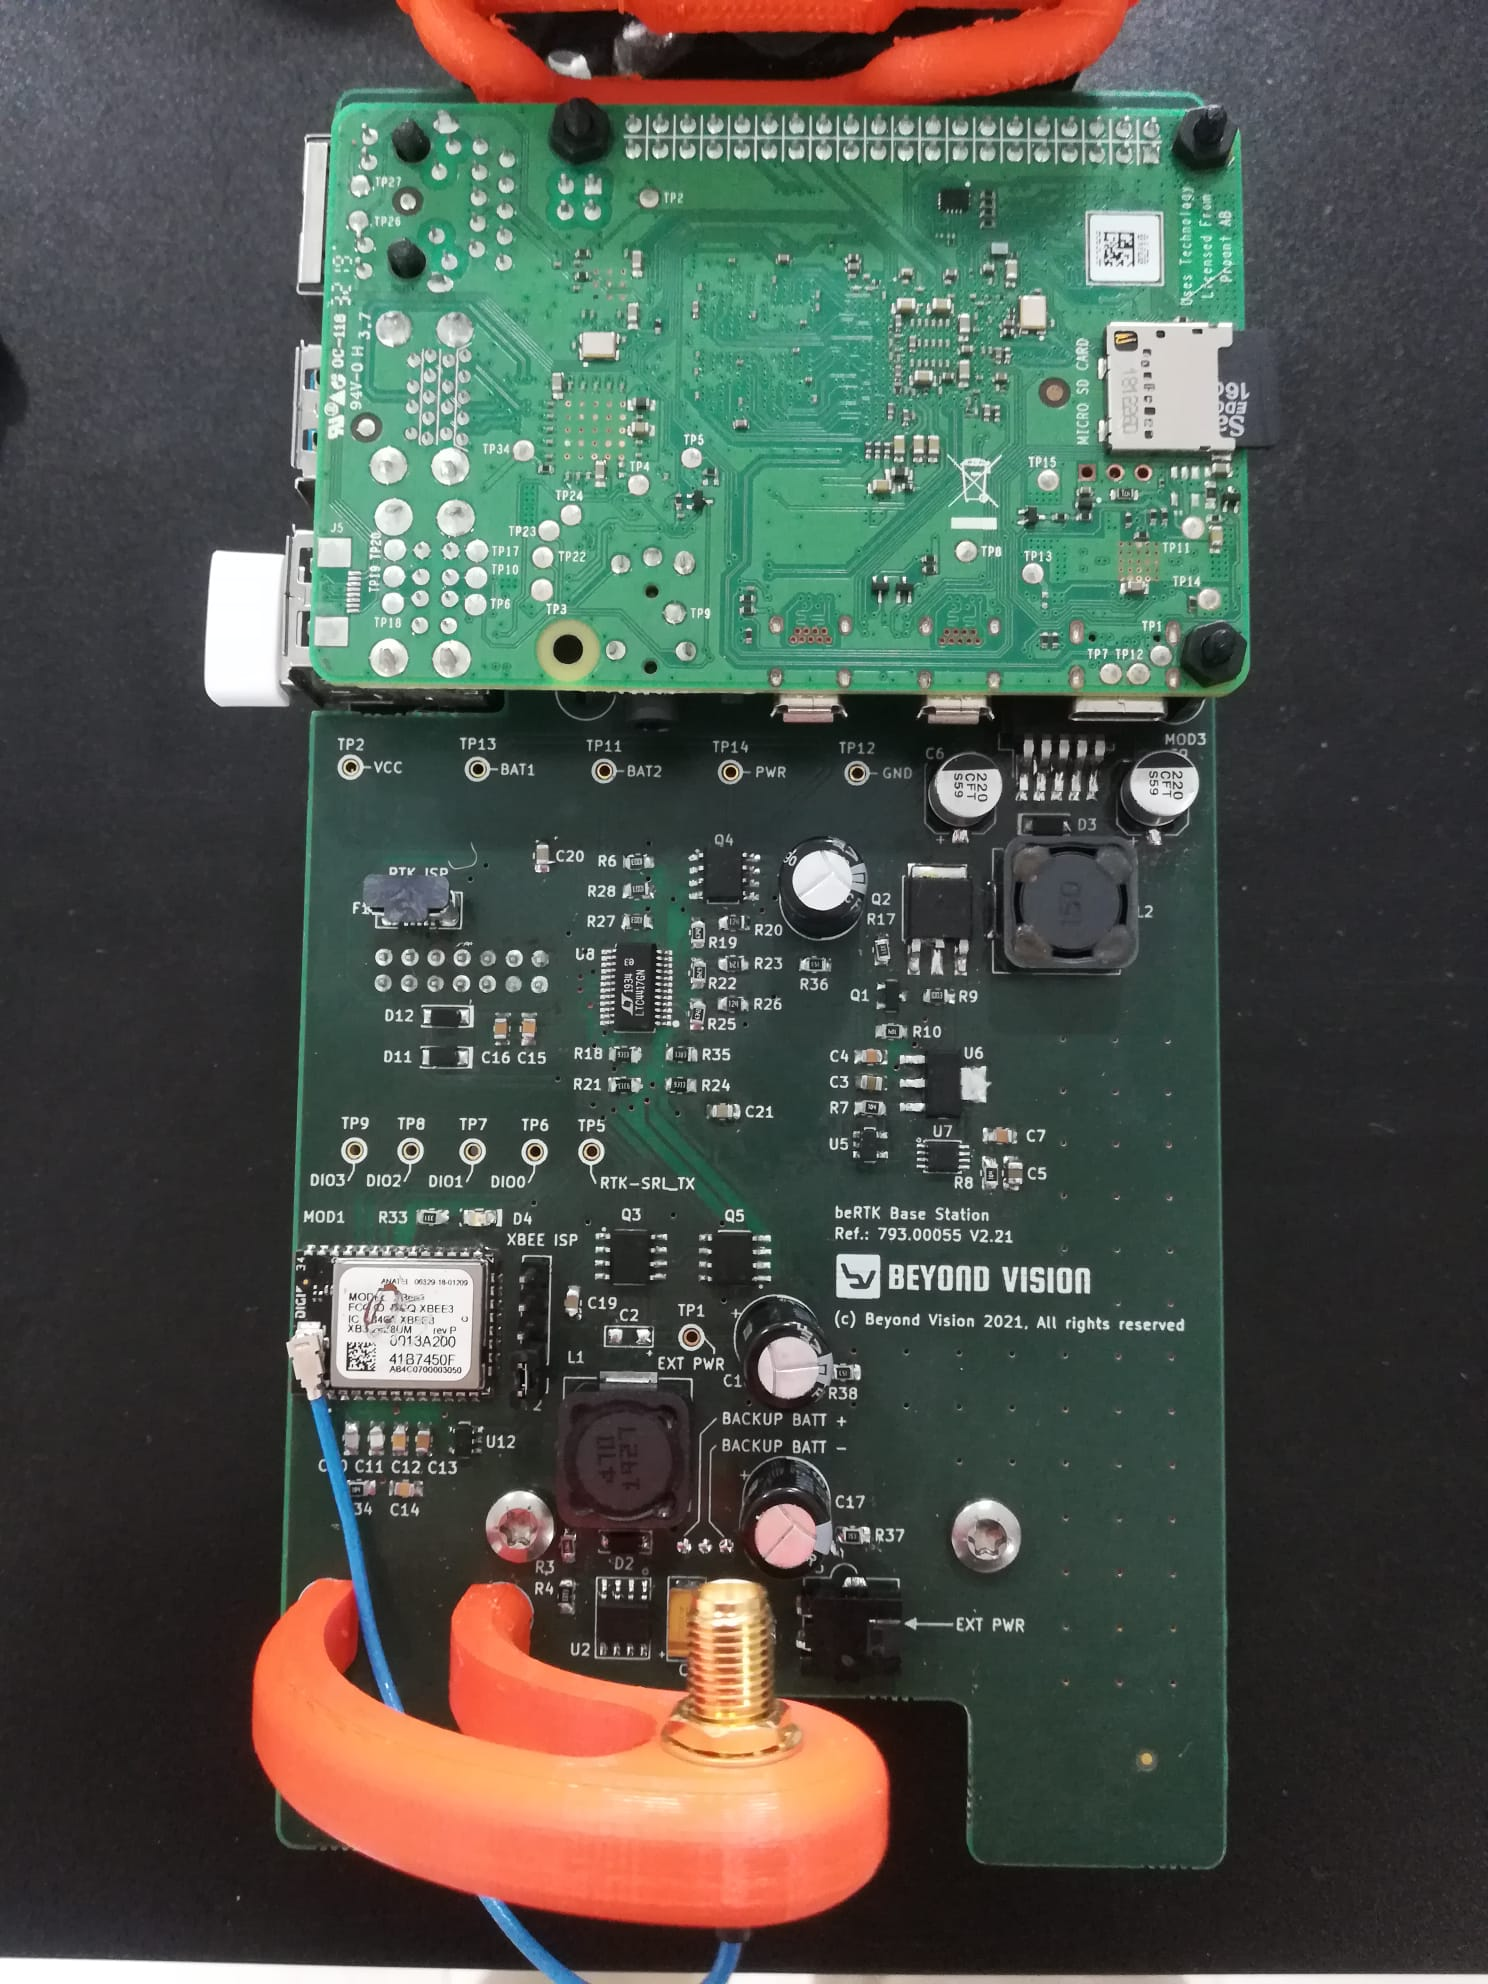
\includegraphics[width=0.5\textwidth, keepaspectratio]{Chapters/Figures/Intro/old_BS.jpeg}
	\caption{Old base station.}
	\label{fig:old_BS}
\end{figure}

This is Figure \ref{fig:old_BS}. It shows the current \gls{base_station}.

\section{Section 1.1}\label{sub:sub1_1}

\section{Section 1.2}\label{sec:sub1_2}

\section{Section 1.3}\label{sec:sub1_3}

\section{Section 1.4}\label{sec:sub1_4}
